\Minisec{Link-State-Routing}
\Minisec{Dijkstra}
\begin{minipage}[t]{0.25\textwidth}
Menge M:=schon abgearbeitete Knoten; \\
Baum B:= gesuchter Quellbaum \\
di:= berechneter Abstand zu Ni \\
 
\textbf{initialisiere: }\\
Startknoten in M und B einfügen, \\
di=Wert der Kante Ni zu Startknoten, sonst $\infty$

\textbf{Bis alle Knoten in M sind: }
\begin{enumerate}
\item \textcolor{red}{suche das kleinste di, }
\item füge diesen Knoten Ni zu M hinzu, 
\item füge die kürzeste Kante von B zu Ni in B ein.
\item passe die d der Nachbarn von Ni an, wenn di + Kante von Ni kürzer ist
\end{enumerate}

\end{minipage}
\begin{minipage}[t]{0.25\textwidth}
Bsp: Startknoten: $N_1$\\
\begin{tabular}{|l|l|c|c|c|}
\hline
Runde 	&	M 			& $d_2$		& $d_3$			& $d_4$\\	\hline
1	&	{$N_1$} 	& \textcolor{red}{1}	& 3 &	 $\infty$ \\ \hline
2	&	{$N_1$, $N_2$} 	&  		& 	\textcolor{red}{2}	 & 3 \\ \hline
3	&	{$N_1$, $N_2$, $N_3$} 	& 		& 	 & \textcolor{red}{3} \\ \hline
\end{tabular}\\
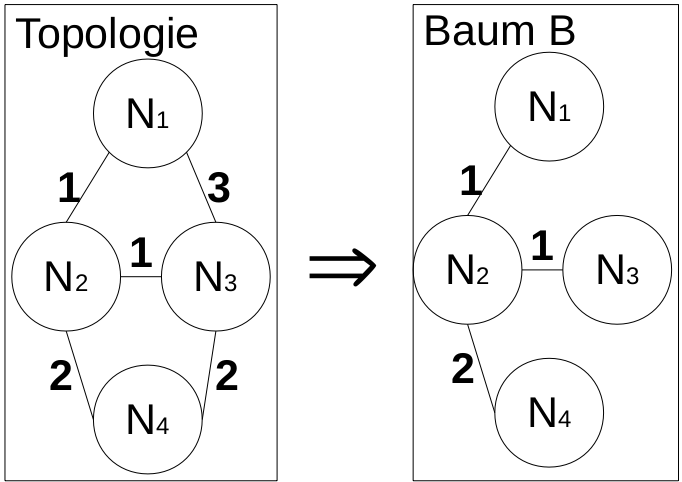
\includegraphics[width=\textwidth]{Dijkstra}
\end{minipage}\\\\

\begin{minipage}{0.25\textwidth}
\Minisec{OLSR - MPR}
Fluten nur an ausgewählte Nachbarn.\\
N(K):= Nachbarn von K \\
N2(K):= Nachbarsnachbarn von K \\
MPR(K):= Weiterflutende knoten in N(K)
\end{minipage} 			
\begin{minipage}{0.25\textwidth}
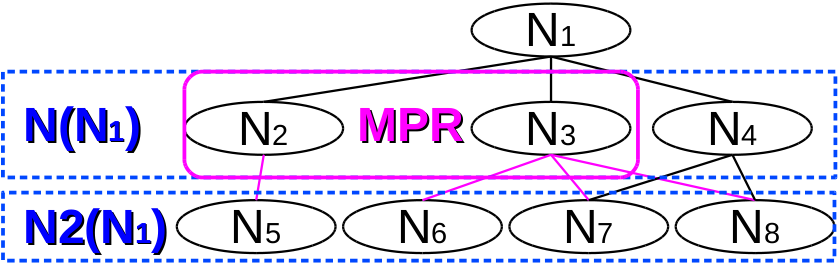
\includegraphics[width=\textwidth]{OLSR}
\end{minipage} 

\begin{enumerate}
\item MPR = Knoten in N(K), die einzige Verbindung eines Knotens in N2(K) sind (Bsp: $N_2$)
\item Solange noch nicht alle Knoten in N2 erreicht werden:\\
Suche den Knoten aus N(K), der die meisten fehlenden Knoten in N2(K) erreicht und füge ihn zu MPR hinzu ($N_3$) \\
(bei mehreren Kandidaten denjenigen mit meisten Nachbarn)
\item Entferne Knoten, wenn danach immer noch alle Knoten in N2(K) erreicht werden
\end{enumerate}

\Minisec{Link-Reversal-Routing}
Weg zu einem Ziel: Directed Acyclic Graph (DAG)\\
\begin{minipage}{0.5\textwidth}
\begin{enumerate}
\item Full Reversal: hat ein Knoten nur eingehende Kanten: drehe alle um
\item Partial Reversal (listenbasiert): Knoten führen Liste über von Nachbarn gedrehte Kanten; sind alle Kanten drin lösche die Liste\\
gibt es nur eingehende Kanten drehe alle Kanten um, die nicht in der Liste stehen; 
\end{enumerate}
\end{minipage}




\Minisec{DBF:}
Jeder Knoten hat eine Tabelle mit Ziel, Hop zum Ziel, Metrik(Kosten);\\
\begin{minipage}{0.5\textwidth}
\begin{tabbing}
\textbf{Initialisierung:} \= Loopback mit Metrik 0 eintragen;\\
\> Verbindung zu den Nachbarn mit der gemessenen Metrik eintragen\\
\> Alle Anderen Verbindungen: Hop = ? Metrik= $\infty$
\end{tabbing}
\end{minipage}

\textbf{Abgleich mit Nachbartabelle:} In jeder Zeile prüfen: \\
\begin{minipage}{0.5\textwidth}
\begin{itemize}
\item Berechne Eintrag der Nachbartabelle + Verbindungsmetrik
\item Ist der Nachbar der Hop der Zeile: Übernimm veränderten Wert
\item Ist die Route über den Nachbarn besser $\rightarrow$ Nachbarn als Hop mit Metrik eintragen
\end{itemize}
\end{minipage}

\textbf{Count-To-Infinity-Problem:} nach Verbindungsabbruch evtl. Feedback-Schleife  \\
\begin{minipage}{0.5\textwidth}
\begin{itemize}
\item definiere kleinen Wert als Unendlich
\item Split Horizon: Zeilen werden nicht dem eingetragenen Hop weitergereicht 
\item Versionsnummern der Einträge (DSDV)
\end{itemize}
\end{minipage}\\

\Minisec{DSDV:}
DBF Tabelle um Spalte für Sequenznummer erweitern (mit -1 initialisiert)

\textbf{Abgleich mit Nachbartabelle:} \underline{höhere} Sequenznummer gewinnt (\underline{Gleiche:} siehe DBF)

\textbf{Nach Abgleich mit allen Nachbarn} :  \textit{Eigene} Sequenznummer +2 ~~(Metrik=0);\\
\textbf{ Verbindungsabbruch} zu Nachbarn Nx: in alle Zeilen mit Hop = Nx: \\
\rule{1cm}{0pt} Metrik = $\infty$ Hop = ? Sequenznummer++





\Minisec{IPv6}
Adressen: 8 4er-Blöcke(Hex) z.B. 47cd::22:1234:a456:12 \\
64 Bit Präfix(Netzwerkanteil) 64 Bit Interface Identifier\\
\begin{tabular}{|c|c|}
\hline
Adressen & Funktion \\ \hline
::1 		& Local Loopback \\ \hline
fe80::/10 	& Link Local Unicast (Autokonfiguration) \\ \hline
fc00::/7	& Unique Local Unicast (Private Adressen) \\ \hline
ff00::/8	& Multicast (Broadcast mit verschiedenen Reichweiten) \\ \hline
weitere:	& Anycast (Route an irgendeinen Host einer speziellen Gruppe) \\ \hline
\end{tabular}\\

\textbf{Autoconfiguration: }\\
\begin{minipage}{0.5\textwidth}
\begin{enumerate}
\item Berechne Identifier (aus MAC oder zufällig)
\item => frage bei Router mit fe801::/64 + Identifyer (Link Local Unicast Adresse)
\item Router teilt mögliche Präfixe mit
\item Host prüft ob Adresse schon vorhanden (Double Address Detection)
\end{enumerate}
\end{minipage}\\


\textbf{DHCP: }\\
\begin{minipage}{0.5\textwidth}
\begin{enumerate}
\item Client: DHCPDISCOVER (per Broadcast)
\item Server: DHCPOFFER 
\item Client: DHCPREQUEST
\item Server: DHCPACK (Client hat nun Adresse geleast)
\end{enumerate}
\end{minipage}
\clearpage




\tabsec{IPv4} Hostanteil $1\dots1$= Broadcast  $0\dots0$= Netzadresse \\
\begin{tabular}{|c|c|c|c|}	
\hline
Klasse & Von & bis &  \\
\hline
A 	& 0.0.0.0 	& 127.255.255.255 & 16.777.214 Hosts	\\
\hline
B	& 128.0.0.0 & 191.255.255.255 & 65.534 Hosts		\\
\hline
C	& 192.0.0.0 & 223.255.255.255 & 254	Hosts	\\
\hline
D	& 224.0.0.0 & 239.255.255.255 & Multicast 	\\
\hline
E	& 240.0.0.0	& 255.255.255.255 & Reserviert 	\\
\hline	
 & 127.0.0.0 & 127.255.255.255 & Loopback 	\\
 \hline
A & 10.0.0.0 & 10.255.255.255 & privat 	\\
 \hline
B & 172.16.0.1 & 172.31.255.255& privat  	\\
 \hline
C & 192.168.0.1 & 192.168.255.255 & privat  	\\
 \hline
\end{tabular}~~~~
\begin{tabular}{|c|c|}
\hline
Oktett & Bits \\ \hline
255 & 1111 1111 \\ \hline
254 & 1111 1110 \\ \hline
252 & 1111 1100 \\ \hline
248 & 1111 1000 \\ \hline
240 & 1111 0000 \\ \hline
224 & 1110 0000 \\ \hline
192 & 1100 0000 \\ \hline
128 & 1000 0000 \\ \hline
\end{tabular}

\minisec{Fragmentieren}
Ident(16Bit) ID eines \underline{Pakets}, Offset(13Bit): Position des Fragments \textbf{\textcolor{red}{/ 8}}	\\
Fragmentierungsbit: 1=verboten, More: 1=weitere , 0=letztes Fragment	

\minisec{Vorgehen}
Größtmögliche Pakete herausschneiden, evtl ein kleinerer Rest im letzten Paket.\\
\textbf{Beachten:} Fragmentieren auf \textcolor{red}{Vielfache von 8} z.B. 512,520... u.U. IP-Header 20Byte \\
Router "defragmentieren" \textbf{nicht}; 
